\subsection{¿Quiénes somos?}


\begin{table}[!hbt]
\begin{tblr}{c c}
    \SetCell[r=10]{} 
\includegraphics[width=0.35\textwidth]{preambulo/Imagen de WhatsApp 2023-10-14 a las 18.27.44_028dad0b.jpg} 
    & \SetCell[r=1]{l} Ivan Ezequiel Cenyko
    &  \\ 
    &  \\
    & \SetCell[r=1]{l}DNI: 46.028.174
    & \\ 
    &  \\
    & \SetCell[r=1]{l}Mail: ivancenyko@gmail.com  
    &  \\
    &  \\
    & \SetCell[r=1]{l}\href{https://www.linkedin.com/in/ivan-cenyko/}{Linkedin: www.linkedin.com/in/ivan-cenyko/}  
    &  \\
    &  \\
        & \SetCell[r=1]{} Programación en microPython y desarrollo web Back-End
    &  \\ 
    &  \\
\end{tblr}
\label{tab:multicol}
\end{table}

\begin{table}[!hbt]
\begin{tblr}{c c}
    \SetCell[r=10]{} 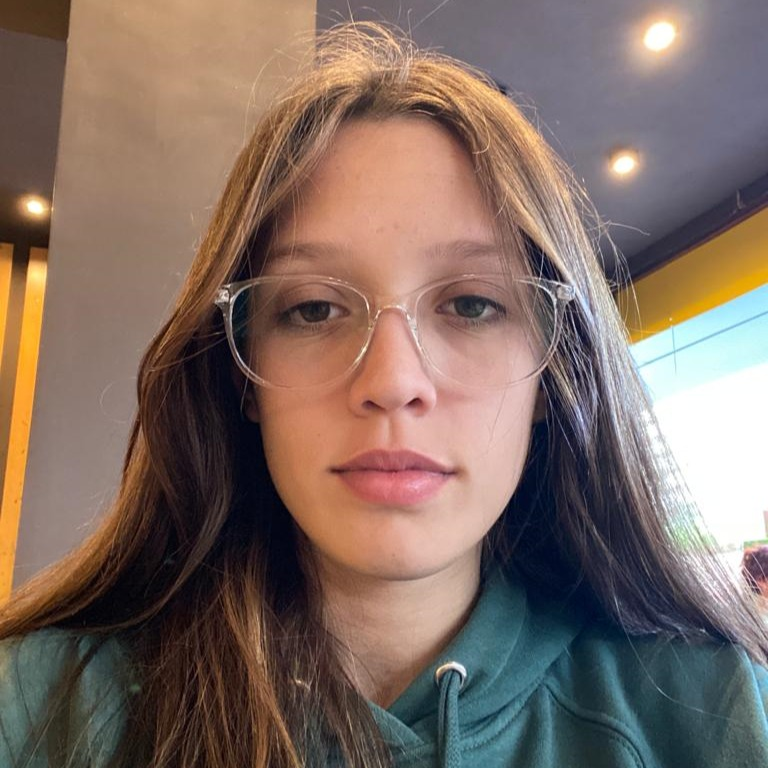
\includegraphics[width=0.35\textwidth]{preambulo/Imagen de WhatsApp 2023-10-14 a las 18.27.45_0fd46106.jpg} 

    & \SetCell[r=1]{l} Lara Paloma Dias
    &  \\ 
    &  \\
    & \SetCell[r=1]{l}DNI: 46200006
    & \\ 
    &  \\
    & \SetCell[r=1]{l}Mail: palomadias308@gmail.com
    &  \\
    &  \\
    & \SetCell[r=1]{l}\href{https://www.linkedin.com/in/lara-paloma-dias-598bb9288/}{Linkedin: www.linkedin.com/in/lara-paloma-dias-598bb9288/}  
    &  \\
    &  \\
    & \SetCell[r=1]{l}Desarrollo web Front-End 
    &  \\
    &  \\
\end{tblr}
\label{tab:multicol}
\end{table}

\begin{table}[!hbt]
\begin{tblr}{c c}
    \SetCell[r=10]{} 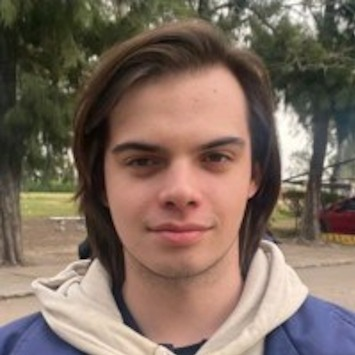
\includegraphics[width=0.35\textwidth]{preambulo/Imagen de WhatsApp 2023-10-14 a las 18.27.45_22ea3b81.jpg} 
    & \SetCell[r=1]{l} Mateo Inza Fior
    &  \\ 
    &  \\
    & \SetCell[r=1]{l}DNI: 46.579.589
    & \\ 
    &  \\
    & \SetCell[r=1]{l}Mail: mateoinzafior@gmail.com
    &  \\
    &  \\
    & \SetCell[r=1]{l}\href{https://www.linkedin.com/in/mateoinzafior/}{Linkedin: www.linkedin.com/in/mateoinzafior/}  
    &  \\
    &  \\
    & \SetCell[r=1]{l}Desarrollo web Front-End y programación en microPython
    &  \\
    &  \\
\end{tblr}
\label{tab:multicol}
\end{table}

\begin{table}[!hbt]
\begin{tblr}{c c}
    \SetCell[r=10]{} 
\includegraphics[width=0.35\textwidth]{preambulo/Imagen de WhatsApp 2023-10-14 a las 18.27.46_242e2534.jpg} 
    & \SetCell[r=1]{l} Agustin Palmieri Hise
    &  \\ 
    &  \\
    & \SetCell[r=1]{l}DNI: 46.364.013
    & \\ 
    &  \\
    & \SetCell[r=1]{l}Mail: aguspalmierihise@gmail.com
    &  \\
    &  \\
    & \SetCell[r=1]{l}\href{https://www.linkedin.com/in/agustin-palmieri-hise/}{Linkedin: www.linkedin.com/in/agustin-palmieri-hise/}  
    &  \\
    &  \\
        & \SetCell[r=1]{l} Diseño y confección eléctrico y electrónico íntegro
    &  \\ 
    &  \\
\end{tblr}
\label{tab:multicol}
\end{table}

\begin{table}[!hbt]
\begin{tblr}{c c}
    \SetCell[r=10]{} 
\includegraphics[width=0.35\textwidth]{preambulo/Imagen de WhatsApp 2023-10-14 a las 18.40.11_fa2abbcb.jpg} 
    & \SetCell[r=1]{l} Maximiliano Nicolas Testa
    &  \\ 
    &  \\
    & \SetCell[r=1]{l}DNI: 46.187.213
    & \\ 
    &  \\
    & \SetCell[r=1]{l}Mail: maxitesta2012@gmail.com  
    &  \\
    &  \\
    & \SetCell[r=1]{l}\href{https://www.linkedin.com/in/maximiliano-testa/}{Linkedin: www.linkedin.com/in/maximiliano-testa/}  
    &  \\
    &  \\
        & \SetCell[r=1]{l} Programación en C y desarrollo Front-End de la Web-app
    &  \\ 
    &  \\
\end{tblr}
\label{tab:multicol}
\end{table}

\begin{figure}[H]
    \centering
    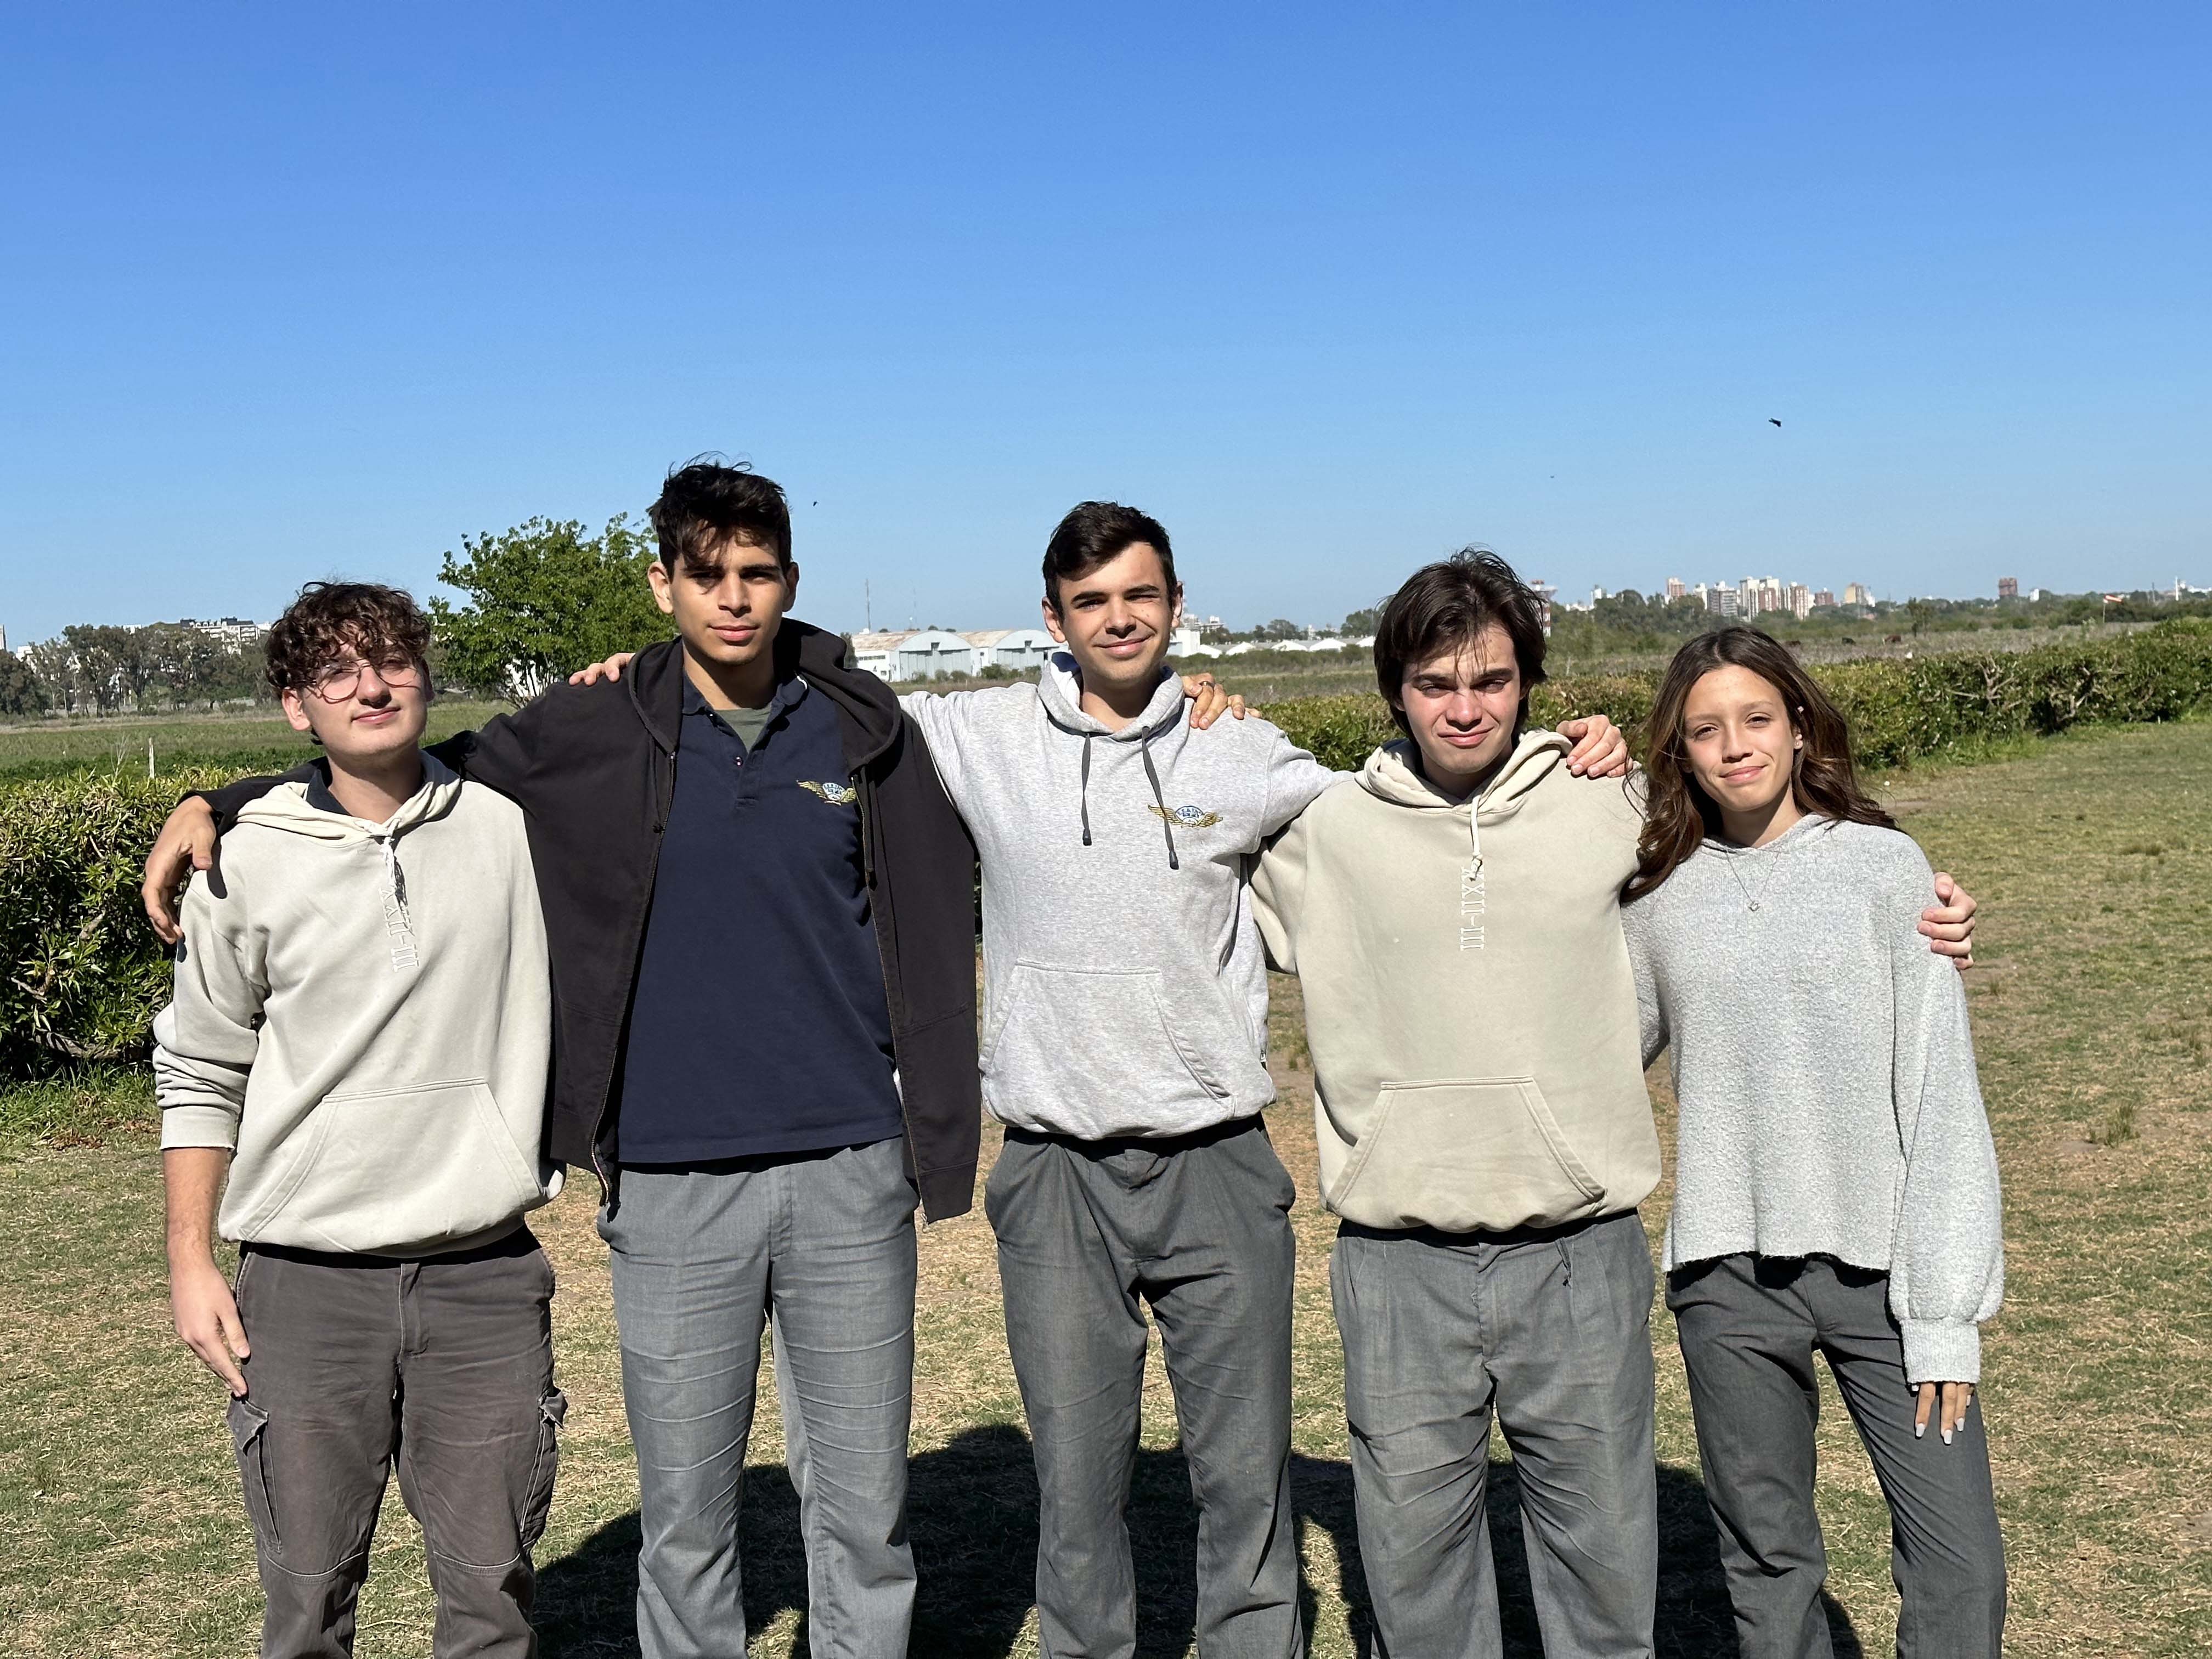
\includegraphics[width=0.85\linewidth]{preambulo/IMG_9428.jpg}
    \caption{Equipo Solar Link}
    \label{fig:equipo solar}
\end{figure}

\begin{figure}[H]
    \centering
    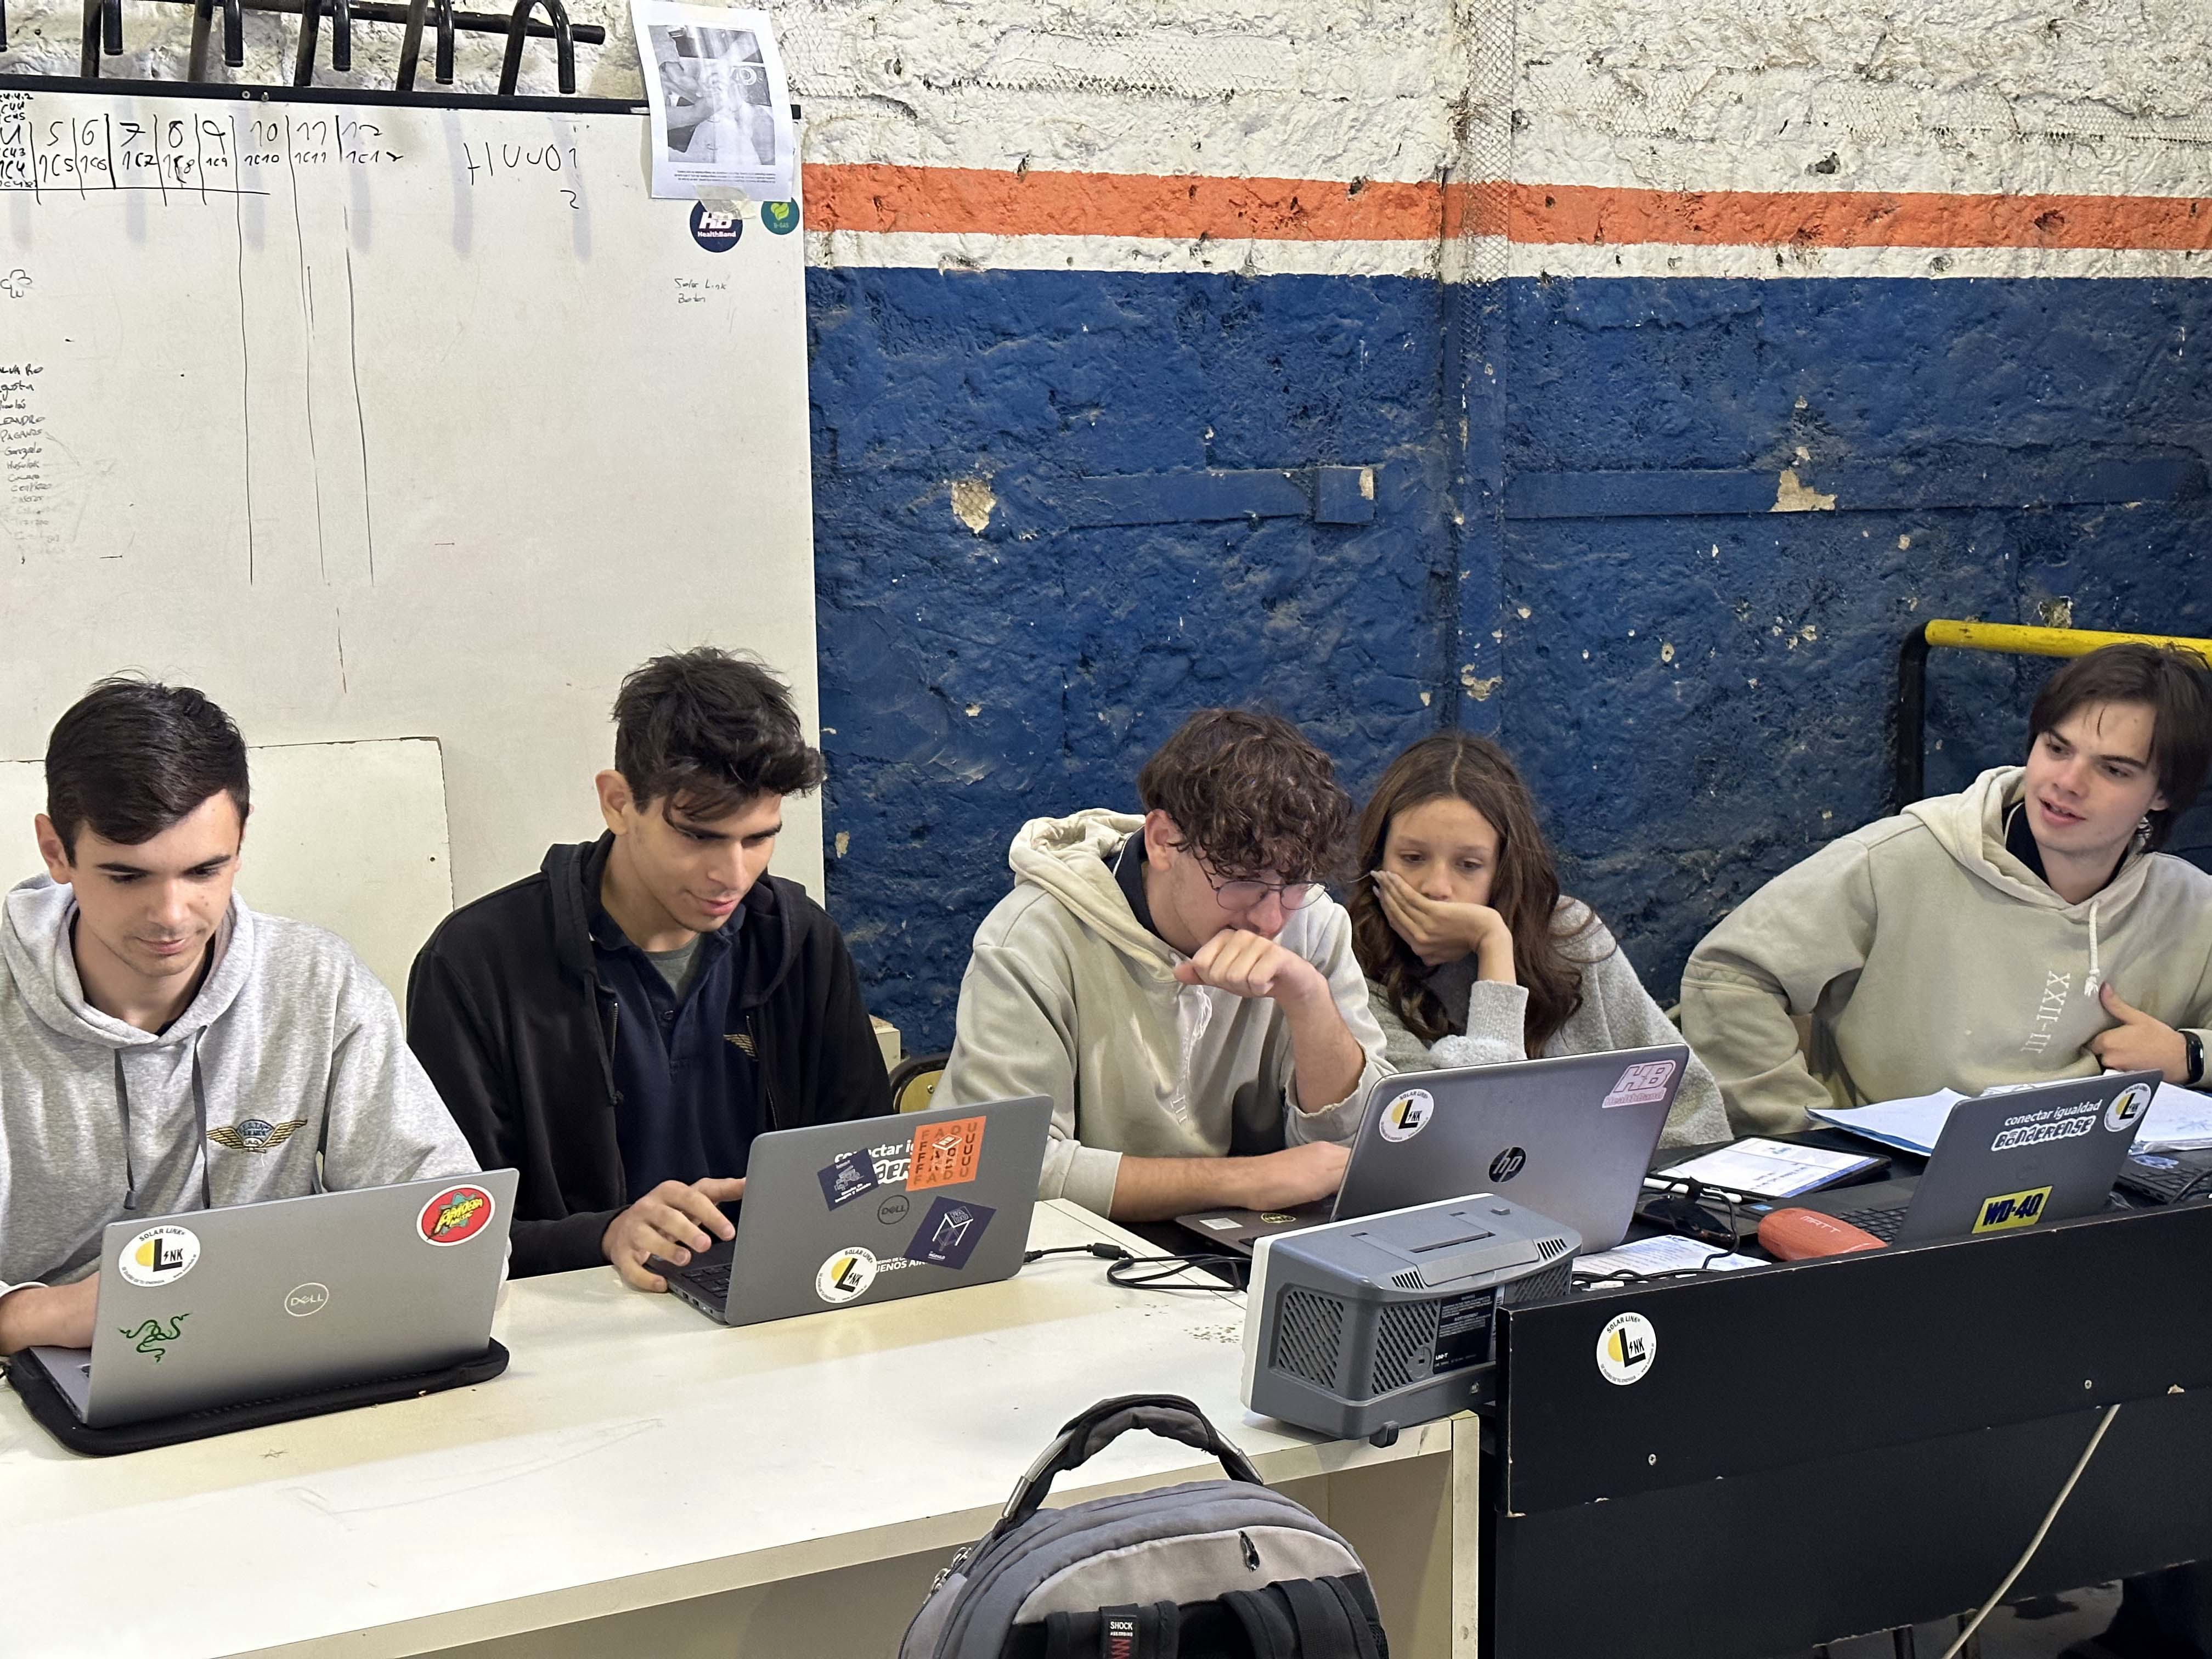
\includegraphics[width=0.85\linewidth]{preambulo/IMG_9439.jpg}
    \caption{Equipo Solar Link trabajando}
    \label{fig:equipo solar laburando}
\end{figure}

\clearpage

\subsection{Contacto}
Podes encontrar a Solar Link en:

\begin{itemize}
\item Mail: info@solarlink.ar
\item Pagina Web: \href{https://www.solarlink.ar}{www.solarlink.ar}
\item Instagram: \href{https://www.instagram.com/solarlink.ar/}{www.instagram.com/solarlink.ar/}
\item Github: \href{https://github.com/solarlink-ar/solarlink}{github.com/solarlink-ar/solarlink}
\item Trello: \href{https://trello.com/w/2023_721c_solarlink}{trello.com/w/2023\_721c\_solarlink}
\end{itemize}

\subsection{Docentes a cargo}

\begin{itemize}
\item Sergio Medina \\ Nos fue de ayuda a la hora de organizar y presentar nuestro proyecto.
\item Fabrizio Carlassara \\ Nos guió en el desarrollo de todo el software del proyecto. 
\item Diego Palmieri \\ Nos prestó las herramientas y los medios necesarios a fin de confeccionar el proyecto.
\end{itemize}

\subsection{Información adicional}

\subsubsection{Tiempo invertido}

\begin{itemize}
\item Fecha de inicio: 20 de noviembre de 2022.
\item Duración: 32 semanas de trabajo.
\item Esfuerzo del proyecto individual: 8 horas de trabajo semanales de cada integrante.
\item Esfuerzo total del proyecto: 1280 horas de trabajo.
\end{itemize}

\subsubsection{Programas utilizados}

\begin{itemize}
\item Visual Studio Code: Fue utilizado como editor de código en diferentes lenguajes.
\item Thonny: Fue utilizado como editor de código para el mirocontroladoor ESP32.
\item KiCad: Fue utilizado para el diseño de todas las PCBs.
\item AutoCad: Fue utilizado para el diseño 3D de las carcasas de las PCBs.
\item Git: Fue utilizado para manejar el código del proyecto entre el grupo.
\item DB Browser: Fue utilizado para leer la base de datos y probar su interacción con lo que programamos.
\item Photoshop: Fue utilizado para el diseño de diferentes imagenes descriptivas del proyecto.
\item Overleaf: Fue utilizado para la realización de la carpeta técnica, de campo y de usuario en LaTex.
\end{itemize}

\subsubsection{Lenguajes de programación y frameworks utilizados}

\begin{itemize}
\item Python: Lógica de página web.
\item MicroPython: Programación del microcontrolador ESP32.
\item C: Programación del microcontrolador Raspberry Pi Pico.
\item Django: Back-end de página web.
\item Microdot: Web de configuración de la ESP32.
\item HTML, CSS: Front-end de la página web.
\item javascript: Front-end de la página web.
\item Terminal de Linux: Manejo de hosting de la web y propósito general.
\item LaTex: Confección de PDFs para carpeta técnica, de campo, y de usuario.
\end{itemize}

\subsection{Agradecimientos}
Este proyecto no hubiera sido posible sin la colaboración de los docentes anteriormente mencionados, la Asociación Cooperadora IMPA y las empresas Eléctrica Bernal, \href{www.bateriasroverano.com.ar}{Roverano}, \href{www.exo.com.ar}{Exo} y \href{www.newtonmicroscopios.com}{Newton Microscopios}.
